\subsubsection{UCA 7 - Autenticazione con credenziali LDAP}%kite level

%\begin{figure}[h]
%	\centering
%	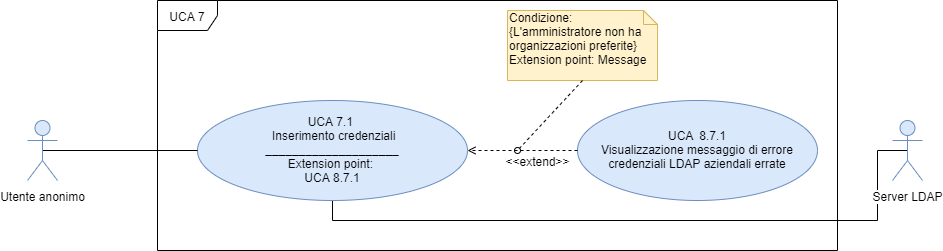
\includegraphics[scale=0.5, center]{sezioni/UseCase/Immagini/UCA7.png}
%	\caption{Tracciamento\ap{G} posizione in un luogo di un'organizzazione\ap{G}}
%\end{figure}

\begin{itemize}
	\item \textbf{Attori primari:} Utente anonimo 
	\item \textbf{Attori secondari:} server LDAP\ap{G} dell'organizzazione.
	\item \textbf{Precondizione:} L'utente autenticato con credenziali Stalker sta per effettuare l'autenticazione con credenziali LDAP.
	\item \textbf{Postcondizione:} L'utente è autenticato all'interno dell'organizzazione\ap{G} con credenziali LDAP.
	\item \textbf{Scenario principale:} L'utente autenticato come utente anonimo effettua l'autenticazione con credenziali LDAP\ap{G} [UCA 7.1] per autenticarsi come utente riconosciuto.
\end{itemize}

\subsubsection{UCA 7.1 - Inserimento credenziali}
\begin{itemize}
	\item \textbf{Attori primari:} Utente anonimo 
	\item \textbf{Attori secondari:} server LDAP\ap{G} dell'organizzazione.
	\item \textbf{Precondizione:} L'utente autenticato con credenziali Stalker inserisce le proprie credenziali LDAP/ap{G}.
	\item \textbf{Postcondizione:} L'utente ha inserito le proprie credenziali LDAP\ap{G}.
	\item \textbf{Scenario principale:}: L'utente inserisce le proprie credenziali LDAP\ap{G} per potersi autenticare.
	\item \textbf{Flusso di eventi:}
	\begin{enumerate}
		\item L'utente inserisci l'indirizzo e-mail [UCA 7.1.1];
		\item L'utente inserisce la password [UCA 7.1.2].
	\end{enumerate}
	\item \textbf{Scenario alternativo:} Il tentativo di autenticazione\ap{G} fallisce perché le credenziali inserite sono errate.
	\item \textbf{Estensioni:}
	\begin{enumerate}
		\item UCA 8.1.7 - Visualizzazione messaggio di errore credenziali errate.
	\end{enumerate}
\end{itemize}

\subsubsection{UCA 7.1.1 - Inserimento indirizzo e-mail}%fish level
\begin{itemize}
	\item \textbf{Attori primari:} Utente anonimo
	\item \textbf{Precondizione:} L'utente inserisce il proprio l'indirizzo e-mail.
	\item \textbf{Postcondizione:} L'utente ha inserito il proprio indirizzo e-mail.
\end{itemize}

\subsubsection{UCA 7.1.2 - Inserimento password}%fish level
\begin{itemize}
	\item \textbf{Attori primari:} Utente anonimo
	\item \textbf{Precondizione:} L'utente inserisci il proprio la password
	\item \textbf{Postcondizione:} L'utente ha inserito la propria password.
\end{itemize}
